\chapter{Le principe d'inertie}
Le fait de savoir pourquoi certains corps sont en mouvement et pas d'autres, savoir si le mouvement ou le repos sont un état \enquote{naturel} ou pas, a beaucoup préoccupé les philosophes et scientifiques de l'Antiquité grecque.

Aristote (384 -- 322 av. J.-C. ), dont la pensée a fortement influencé les sciences jusqu'au Moyen-Âge, suppose que le \enquote{repos} est l'état naturel d'un objet. Par conséquent, toute chose est amenée à retourner à cet état une fois isolée de toute autre influence.

\begin{figure}[h!]
    \centering
    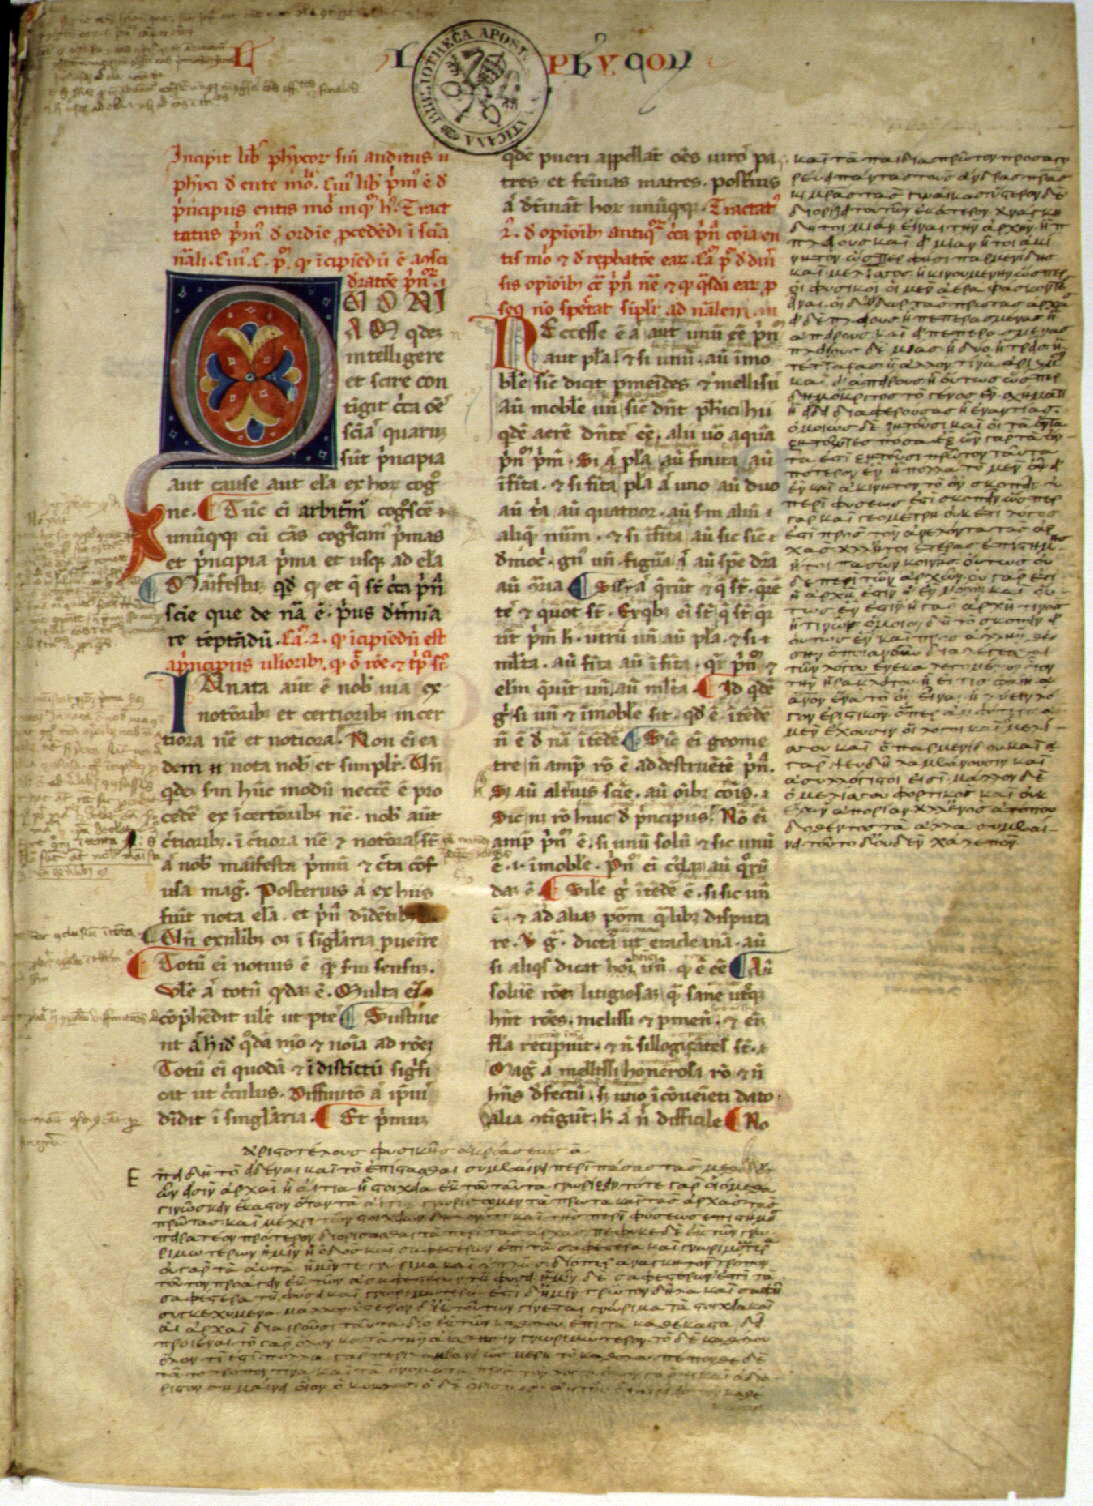
\includegraphics[width=.35 \linewidth]{Aristotle_latin_manuscript.jpg}
    \caption{Manuscrit médiéval de la Physique d'Aristote}
    \label{Aristotle_latin_manuscript}
\end{figure}

\newpage

C'est Galilée (1564 -- 1642) le premier qui énoncera l'idée révolutionnaire pour son époque selon laquelle l'\enquote{état naturel de repos} d'Aristote n'existe pas. C'est d'ailleurs lui qui développe l'idée de relativité du mouvement abordée dans le cours de cinématique.

\begin{figure}[h!]
    \centering
    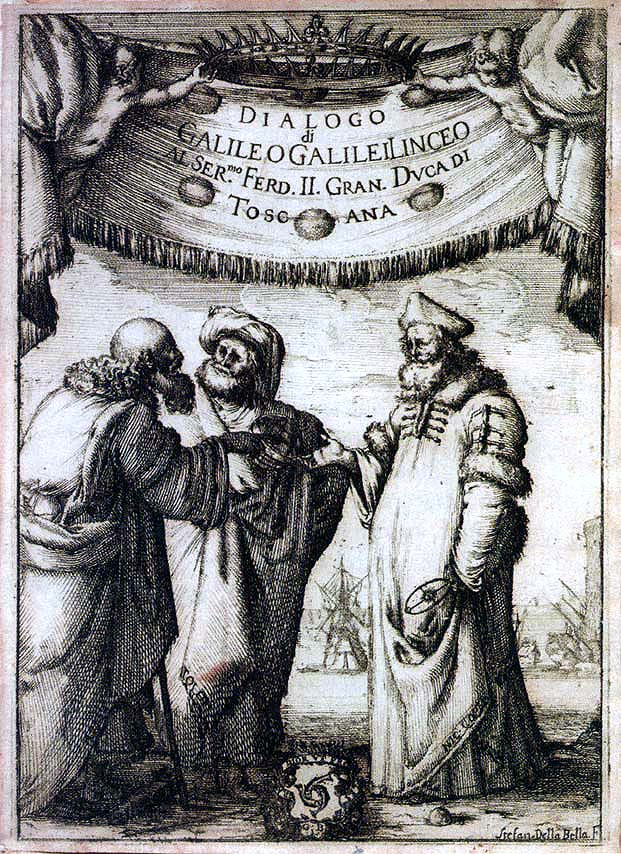
\includegraphics[width=.4 \linewidth]{Galilee_dialogue.jpg}
    \caption{L'ouvrage de Galilée \enquote{Dialogue sur les deux grands systèmes du monde} publié en 1632.}
    \label{Galilee_dialogue}
\end{figure}

C'est finalement Newton qui rependra et reformulera ce concept dans les \enquote{Principia} en 1726.

\newpage



\section{Énoncé du principe d'inertie}
Le principe d'inertie de Newton est très simple, il affirme que :
\begin{encadre}
    Lorsque la force nette qui s'exerce sur un corps est nulle, alors sa vitesse ne varie pas. Ce corps reste donc en MRU ou au repos.
\end{encadre}

Le mouvement en ligne droite et à vitesse constante (MRU) ainsi que le repos sont les états naturels des corps. Il n'est pas possible de distinguer ces deux états et que ceux-ci se maintiennent tant qu'aucune force n'agit sur le corps concerné.

Inversement, le principe d'inertie permet de dire que lorsqu'un corps est au repos ou en MRU, alors la somme des forces qui s'exerce dessus est nulle.

\begin{encadre}
    \motcle{Principe d'inertie}

    \(\sum{\vec{F}} = \vec{0} \leftrightarrow \Delta \vec{v}=\vec{0}\)
\end{encadre}

\newpage

\section{Les forces de frottement}
Si Aristote estimait que tous les objets retournent naturellement vers un état de repos, c'est sans doute parce que c'est ce qu'on observe le plus souvent ! Lorsque tu roules à vélo sur un terrain plat, si tu arrêtes de pédaler, le vélo finit effectivement par s'arrêter.

Cette situation s'explique par l'existence de forces de frottement entre les roues et le sol, entre le cycliste, le vélo et l'air, entre les roues et leur axe de rotation. Ce sont ces forces qui font varier la vitesse du vélo.

Les forces de frottement sont omniprésentes et elles permettent d'expliquer un grand nombre de situations de repos ou de variation de vitesse. Elles devront toujours être prises en compte lorsqu'on réalise un bilan dans le cadre du principe d'inertie.

\section{Applications}
\begin{exercise}
    Une personne se tient debout dans un bus sans se tenir à une main courante. Le bus freine brusquement.
    \begin{enumerate}[a)]
        \item Que va-t-il se passer ?
        \item Comment expliques-tu ce qui se passe ?
    \end{enumerate}
\end{exercise}

\begin{exercise}
    Une voiture roule à vitesse constante. Explique pourquoi il est tout de même nécessaire de faire fonctionner le moteur.
\end{exercise}

\begin{exercise}
    Une sonde spatiale se déplace loin de toutes planètes. A-t-elle besoin d'un moteur pour maintenir sa vitesse ?
\end{exercise}

\begin{exercise}
    Une nappe est posée sur une table. Sur la nappe, se trouve une assiette. On tire brusquement sur la nappe, que pourrais-tu observer ?
\end{exercise}

\begin{exercise}
    Quel est l'intérêt d'une ceinture de sécurité ?
\end{exercise}

\begin{exercise}
    Une décoration est attachée au rétroviseur intérieur d'une voiture.
    \begin{enumerate}
        \item Comment se comporte la décoration lorsque la voiture tourne vers la droite ?
        \item Explique ce comportement.
    \end{enumerate}
    \begin{figure}[h!]
        \centering
        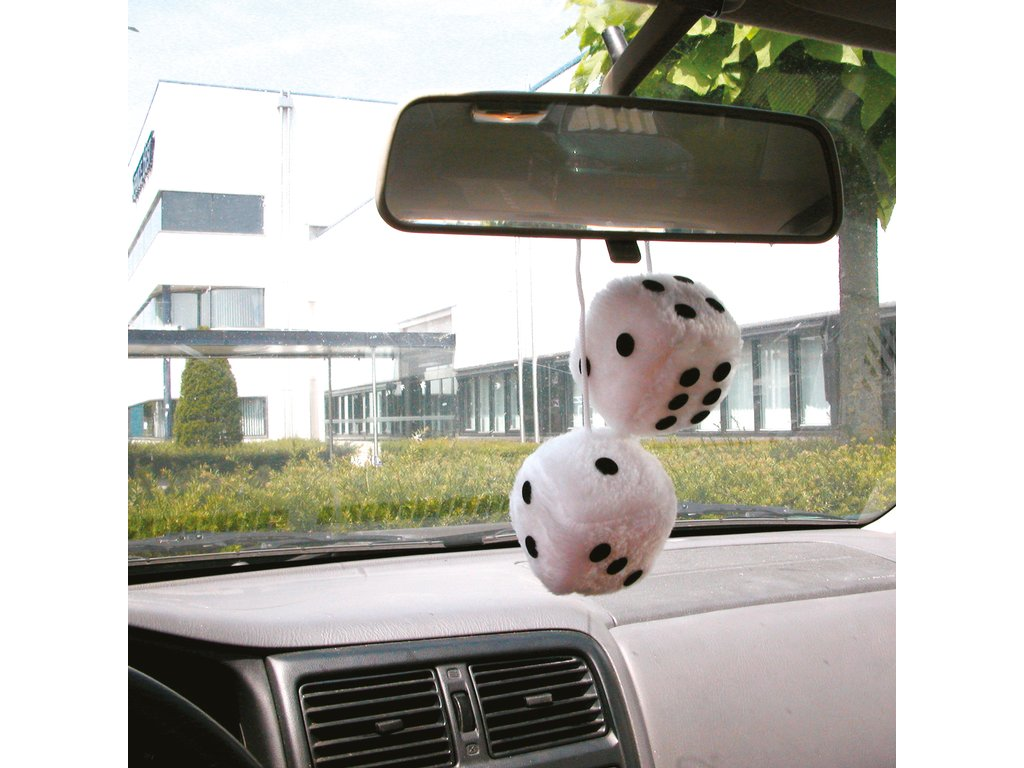
\includegraphics[width=.5 \linewidth]{des_retroviseur.jpg}
        \label{des_retroviseur}
    \end{figure}
\end{exercise}